\subsection{Redes neuronales}
\begin{frame}{Métodos supervisados}
\begin{columns}
\begin{column}{0.9\textwidth}
Una red neuronal artificial es un modelo predictivo basado en el funcionamiento del cerebro humano.\\ 
Cada neurona recibe la información de las neuronas anteriores, las procesa y manda la señal de salida  a las neuronas siguientes. \\

La ventaja es que este tipo de modelos se pueden escalar para tener la complejidad que requieran los datos a costa de perder interpretabilidad, es por ello que normalmente se utilizan con fines únicamente predictivos. 
\end{column}
\end{columns}
\end{frame}

\begin{frame}{Métodos supervisados}
\begin{columns}
\begin{column}{0.9\textwidth}
Conceptos principales: 
\begin{itemize}
\item Pesos sinápticos.
\item Función de activación.
\item Neurona artificial.
\end{itemize}
\begin{figure}[h]
  \centering
  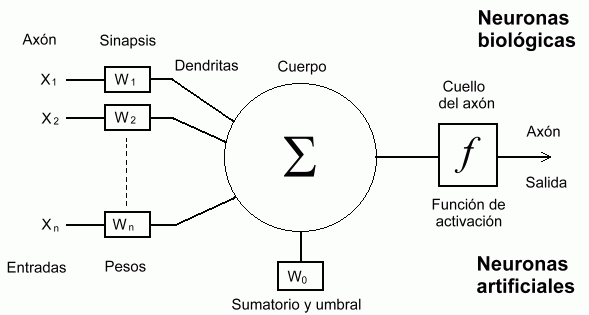
\includegraphics[scale=0.45]{Documentos Extra/Imagenes/neurona.png}
  \caption{Analogía neurona biológica y artificial procedente de \url{https://www.um.es/LEQ/Atmosferas/Ch-VI-3/F63s4p3.htm}}
  \label{fig:neurona}
\end{figure}

\end{column}
\end{columns}
\end{frame}

\begin{frame}{Métodos supervisados}
\begin{columns}
\begin{column}{0.9\textwidth}
Tipos de capas: 
\begin{itemize}
\item Capas de entrada.
\item Capa oculta.
\item Capa de salida.
\end{itemize}

\begin{figure}[h]
  \centering
  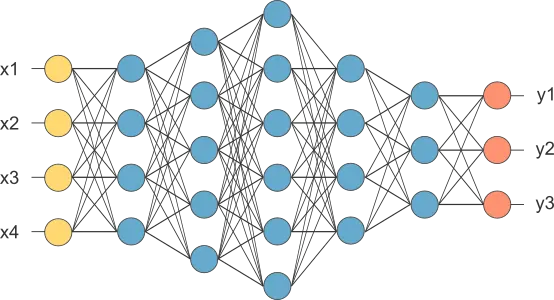
\includegraphics[scale=0.3]{Documentos Extra/Imagenes/red-neuronal-grande.png}
  \caption{Estructura de una red neuronal como un grafo procedente de \url{https://www.neuraldesigner.com/learning/tutorials/neural-network}}
  \label{fig:red neuronal}
\end{figure}
\end{column}
\end{columns}
\end{frame}

\begin{frame}{Métodos supervisados}
\begin{columns}
\begin{column}{0.9\textwidth}
El ajuste de las redes neuronales se realiza con un proceso llamado \emph{backpropagation}. El proceso consiste en los siguientes pasos 
\begin{itemize}
\item Se inicia el modelo con un conjunto de parámetros que puede ser aleatorio o prefijados por el usuario. 
\item Se evalúa la red neuronal con esos parámetros. 
\item Se actualizan los parámetros de acuerdo a algún método de optimización como puede ser el método del gradiente. 
\item Se repiten los dos pasos anteriores hasta que se alcanza algún criterio de parada. 
\end{itemize} 
\end{column}
\end{columns}
\end{frame}

